\section{\gls{DPR} for External Fault Mitigation}\label{ExternalFaults}
Redundancy is a necessary feature to increase the dependability of a system.
Systems that have a need for high dependability encompass e.g. any safety critical system where a fault can result in the harm or even loss of human live.
Systems where maintenance may be difficult or expensive are another set of examples where redundancy is useful.
Redundancy can be achieved through the provision of multiple hardware entities that perform the same task.
If one hardware entity fails, another can take over and supply the expected functionality.
This can get expensive when there are multiple smaller hardware entities that perform specific computational work. 
To reduce space usage and cost, a general purpose \gls{CPU} can be used.
This \gls{CPU} can then emulate the functionality of the faulty hardware and thereby mitigates the fault. 
But this approach introduces new margin for error, as a two-pronged development may lead to discrepancies.
Another issue are real-time requirements that need to be fulfilled.
A regular \gls{CPU} may not be able to provide concurrent computations or the required performance, as the emulated hardware (or software) may be too complex.

A solution to these problems is the usage of \glspl{FPGA} as a means of redundancy. 
As the \gls{FPGA} can be reconfigured with different functionality during runtime, it reduces the total amount of hardware that is needed to achieve redundancy.
Unlike \glspl{CPU}, \glspl{FPGA} provide better means for concurrent computation and are suitable to emulate multiple faulty hardware entities in a more appropriate manner. %TODO: Citation needed

\begin{figure}
    \resizebox{\columnwidth}{!}{

\tikzset{every picture/.style={line width=0.25pt}} %set default line width to 0.75pt        

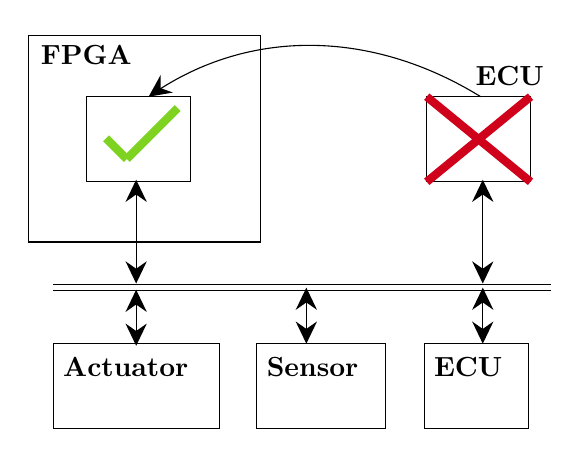
\begin{tikzpicture}[x=0.75pt,y=0.75pt,yscale=-1,xscale=1]
%uncomment if require: \path (0,279); %set diagram left start at 0, and has height of 279

%Shape: Rectangle [id:dp5787797491333819] 
\draw   (8,20.5) -- (120,20.5) -- (120,120) -- (8,120) -- cycle ;
%Shape: Rectangle [id:dp17505095690594463] 
\draw   (36,50) -- (86,50) -- (86,91) -- (36,91) -- cycle ;
%Shape: Rectangle [id:dp004684645465554249] 
\draw   (20,169) -- (100,169) -- (100,210) -- (20,210) -- cycle ;
%Shape: Rectangle [id:dp2725857150503048] 
\draw   (118,169) -- (180,169) -- (180,210) -- (118,210) -- cycle ;
%Shape: Rectangle [id:dp2885393682660524] 
\draw   (200,50) -- (250,50) -- (250,91) -- (200,91) -- cycle ;
%Shape: Rectangle [id:dp4969175268738504] 
\draw   (199,169) -- (249,169) -- (249,210) -- (199,210) -- cycle ;
%Straight Lines [id:da8580754234796655] 
\draw [color={rgb, 255:red, 208; green, 2; blue, 27 }  ,draw opacity=1 ][line width=3]    (200,50) -- (250,91) ;


%Straight Lines [id:da5772916268060835] 
\draw [color={rgb, 255:red, 208; green, 2; blue, 27 }  ,draw opacity=1 ][line width=3]    (250,50) -- (200,91) ;


%Curve Lines [id:da5702734861080319] 
\draw    (68.1,48.54) .. controls (114.3,17.01) and (173.3,17.5) .. (226,50) ;

\draw [shift={(66,50)}, rotate = 324.64] [fill={rgb, 255:red, 0; green, 0; blue, 0 }  ][line width=0.75]  [draw opacity=0] (10.72,-5.15) -- (0,0) -- (10.72,5.15) -- (7.12,0) -- cycle    ;
%Straight Lines [id:da7282259837027933] 
\draw [color={rgb, 255:red, 126; green, 211; blue, 33 }  ,draw opacity=1 ][line width=3]    (80,55.5) -- (55.5,80) ;


%Straight Lines [id:da7142424530641487] 
\draw [color={rgb, 255:red, 126; green, 211; blue, 33 }  ,draw opacity=1 ][line width=3]    (55.5,80) -- (45.5,70) ;


%Straight Lines [id:da36465994520752654] 
\draw    (20,140.5) -- (260,140.5)(20,143.5) -- (260,143.5) ;


%Straight Lines [id:da9447465253235761] 
\draw    (227,92) -- (227,138) ;
\draw [shift={(227,140)}, rotate = 270] [fill={rgb, 255:red, 0; green, 0; blue, 0 }  ][line width=0.75]  [draw opacity=0] (10.72,-5.15) -- (0,0) -- (10.72,5.15) -- (7.12,0) -- cycle    ;
\draw [shift={(227,90)}, rotate = 90] [fill={rgb, 255:red, 0; green, 0; blue, 0 }  ][line width=0.75]  [draw opacity=0] (10.72,-5.15) -- (0,0) -- (10.72,5.15) -- (7.12,0) -- cycle    ;
%Straight Lines [id:da358175601755349] 
\draw    (60,92) -- (60,138) ;
\draw [shift={(60,140)}, rotate = 270] [fill={rgb, 255:red, 0; green, 0; blue, 0 }  ][line width=0.75]  [draw opacity=0] (10.72,-5.15) -- (0,0) -- (10.72,5.15) -- (7.12,0) -- cycle    ;
\draw [shift={(60,90)}, rotate = 90] [fill={rgb, 255:red, 0; green, 0; blue, 0 }  ][line width=0.75]  [draw opacity=0] (10.72,-5.15) -- (0,0) -- (10.72,5.15) -- (7.12,0) -- cycle    ;
%Straight Lines [id:da07393951188629155] 
\draw    (60,145) -- (60,168) ;
\draw [shift={(60,170)}, rotate = 270] [fill={rgb, 255:red, 0; green, 0; blue, 0 }  ][line width=0.75]  [draw opacity=0] (10.72,-5.15) -- (0,0) -- (10.72,5.15) -- (7.12,0) -- cycle    ;
\draw [shift={(60,143)}, rotate = 90] [fill={rgb, 255:red, 0; green, 0; blue, 0 }  ][line width=0.75]  [draw opacity=0] (10.72,-5.15) -- (0,0) -- (10.72,5.15) -- (7.12,0) -- cycle    ;
%Straight Lines [id:da8542656416019287] 
\draw    (142,144) -- (142,167) ;
\draw [shift={(142,169)}, rotate = 270] [fill={rgb, 255:red, 0; green, 0; blue, 0 }  ][line width=0.75]  [draw opacity=0] (10.72,-5.15) -- (0,0) -- (10.72,5.15) -- (7.12,0) -- cycle    ;
\draw [shift={(142,142)}, rotate = 90] [fill={rgb, 255:red, 0; green, 0; blue, 0 }  ][line width=0.75]  [draw opacity=0] (10.72,-5.15) -- (0,0) -- (10.72,5.15) -- (7.12,0) -- cycle    ;
%Straight Lines [id:da22998818326497883] 
\draw    (227,144) -- (227,167) ;
\draw [shift={(227,169)}, rotate = 270] [fill={rgb, 255:red, 0; green, 0; blue, 0 }  ][line width=0.75]  [draw opacity=0] (10.72,-5.15) -- (0,0) -- (10.72,5.15) -- (7.12,0) -- cycle    ;
\draw [shift={(227,142)}, rotate = 90] [fill={rgb, 255:red, 0; green, 0; blue, 0 }  ][line width=0.75]  [draw opacity=0] (10.72,-5.15) -- (0,0) -- (10.72,5.15) -- (7.12,0) -- cycle    ;

% Text Node
\draw (36,30) node  [align=left] {\textbf{FPGA}};
% Text Node
\draw (240,40) node  [align=left] {\textbf{ECU}};
% Text Node
\draw (220,180) node  [align=left] {\textbf{ECU}};
% Text Node
\draw (145,180) node  [align=left] {\textbf{Sensor}};
% Text Node
\draw (55,180) node  [align=left] {\textbf{Actuator}};


\end{tikzpicture}
}
    \caption{External Fault Mitigation - functionality from a faulty \gls{ECU} is provided by a module (instantiated with \gls{DPR}) within the \gls{FPGA}}\label{fig:externalFaultMitigation}
\end{figure}

\cite{shanker_enhancing_nodate}, \cite{crdl_fail-safe_nodate}

\subsection{Types of External Faults}
\subsection{Mitigation Strategies for External Faults}